\documentclass{article}

\usepackage[utf8]{inputenc} \usepackage[ngerman]{babel}
\usepackage{graphicx}
\usepackage{amssymb} \usepackage{amsmath}
\usepackage{listings}
\usepackage{color}
\usepackage{latexsym}

\title{Aufgabenblatt 3 - Aufgabe 4}

\author{}

\begin{document}

\maketitle

\begin{enumerate}
\item[(a)]Zwei Yes-Zweige entfallen, da jeweils bereits vorher der selbe Vergleich durchgef\"uhrt wurde. Aufgrund des Bubble-Sort Algorithmus wird der Vergleich dennoch ein zweites mal berechnet.\\
\begin{center}
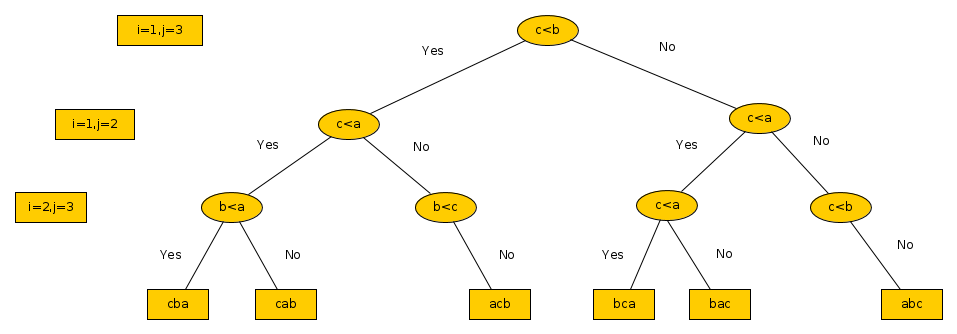
\includegraphics[scale=0.4]{4aGraph.png}\\
\end{center}
\item[(b)]
Damit BUBBLE-SORT im Best-Case in $O(n)$ liegt, kann man den Algorithmus so verändern, dass, wenn in einem Durchlauf der \"au{\ss}eren Schleife keine Elemente vertauscht werden, der Algorithmus abbricht. Dies liefert eine Laufzeit in $O(n)$ bei einer bereits sortierten Eingabe.
\item[(c)]
\begin{lstlisting}
BUBBLESORT(A)
exchanged=true
for i=1 to A.length-1
	if exchanged==true
		exchanged=false
		for j= A.length downto i+1
			if A[j]<A[j-1]
				exchange A[j] with A[j-1]
				exchanged=true
	else leavefor
\end{lstlisting}
\item[(d)]
Bei jedem Durchlauf der \"außeren Schleife, wird nun ein der Vergleich, ob exchanged true ist und die Zuweisung des Wertes false zu exchanged mehr durchgef\"uhrt. Weiterhin wird in der inneren Schleife, ebenfalls eine Wertzuweisung mehr durchgef\"uhrt. \\
Die Laufzeit des Algorithmus wird dadurch nur um einen konstanten Faktor erh\"oht, w\"ahrend sich die Best-Case Laufzeit auf einen Durchlauf durch das Array also $O(n)$ reduziert wird. Somit lohnt sich die Anpassung.
\item[(e)]
Der Baum unterscheidet sich im Zweig ganz rechts. Wenn w\"ahrend i=1 keine Vertauschung durchgef\"uhrt wird, bricht der Algorithmus vor i=2 ab. \\
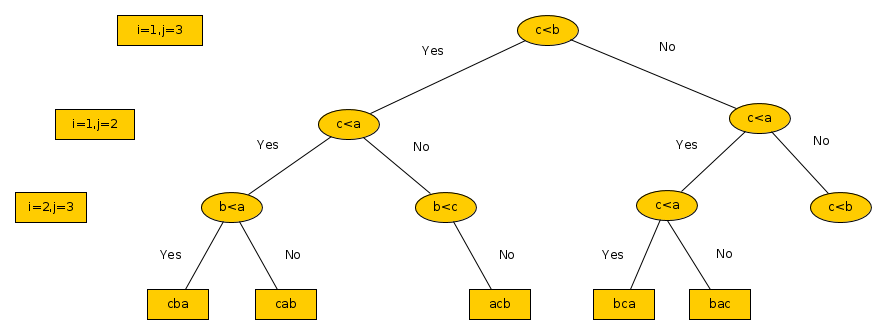
\includegraphics[scale=0.4]{4eGraph.png}\\
\end{enumerate}
\end{document}

